\chapter{Stellar Parameters}\label{chap:introduction}

Despite the fact that iron abundances derived from both excitation levels (Fe I 
and Fe II) are affected by uncertainties in the model atmospheres temperature and
NLTE effects \citep[see][and reference therein]{2017A&A...604A.129M}, many researches still rely on this method (the so-called traditional 
spectroscopic method) to derive their stellar atmospheric parameters. 
Our adopted stellar parameters have been determined through this standard spectroscopic method. 
Additionally, we were able to determine effective temperatures from photometry and surface gravities from parallax/distances.

\section{Effective temperature}
The effective temperatures (\ensuremath{T_\mathrm{eff}}) were estimated by 
minimizing the trend between Fe I lines abundances and excitation potential ($\chi$). 

To estimate \ensuremath{T_\mathrm{eff}}~from the available colors (B, V, J, H, and K), we cross match our sample with two catalogs 
from the Virtual Observatory:  The fourth US Naval 
Observatory CCD Astrograph Catalog (UCAC4, \citealt{2013AJ....145...44Z} )
and Two Micron All Sky Survey (2MASS, \citealt{2006AJ....131.1163S}) and then
employ \citet{2005ApJ...626..465R} temperature calibration.
These \ensuremath{T_\mathrm{eff}}~(determined from photometric and spectroscopic methods) together with \ensuremath{T_\mathrm{eff}}~
taken from Gaia DR2 \citep{2018A&A...616A...1G} are in good agreement with each other ($\pm 150$ K).

\section{Surface gravity and microturbulence}
We determined the surface gravity (\ensuremath{\log\,g}) by forcing Fe I abundances to 
agree with Fe II abundances. In addition, we crossed match our sample with Gaia DR2 distances catalogue \citep{2018AJ....156...58B}, to estimate 
the distance modulus from the available parallax of \citet{2018A&A...616A...1G} (see Eq. \ref{eq:2} and Eq. \ref{eq:3}).



\begin{equation}\label{eq:2}
\log \frac{g}{g_{\odot}} = \log \frac{M}{M_{\odot}} + 4 \log 
\frac{T_{\rm eff}}{T_{\rm eff}} + 0.4(M_{bol} - M_{bol_{\odot}})
\end{equation}


\begin{equation}\label{eq:3}
M_{bol} = V+BC+5 \log \varpi+5
\end{equation}

\begin{figure}[!ht]
\centering
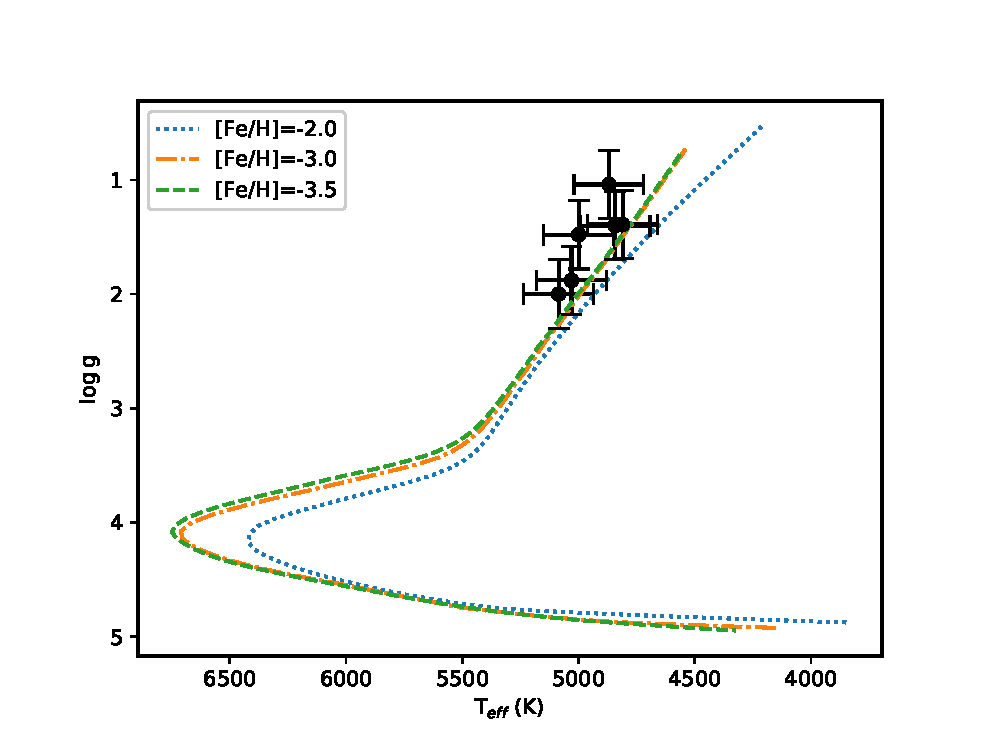
\includegraphics[width=\textwidth, angle=0]{teff_logg.eps}
   \caption{Our sample shown in an H-R-Diagram, based on the \ensuremath{T_\mathrm{eff}} ~and \ensuremath{\log\,g}  determined from the LIKC/APF spectra.
   Yale-Yonsei 12 \Gyr~ isochrones with [$\alpha$/Fe] = +0.4 and [Fe/H] = $-$2.5, $-$3.0, and $-$3.5 from \citet{2004ApJS..155..667D}  overplotted as reference.}
\label{fig:isoch}
\end{figure}


where, $M$ is the stellar mass, $M_{bol}$ is the absolute bolometric magnitude, 
$V$ is the visual magnitude, $BC$ is the bolometric correction \citep[see][Eq. 18]{1999A&AS..140..261A}, and $\pi$ is the parallax.

The microturbulence velocities ($\xi$) were determined by removing any trend between Fe I lines 
abundances with the EWs of those lines. 


The \ensuremath{T_\mathrm{eff}}\,determined from the photometric and spectroscopic methods show 
systematically different results. \citet{2013ApJ...769...57F} have presented an explicit method to adjust the spectroscopic \ensuremath{T_\mathrm{eff}}. 
This scheme increases the \ensuremath{T_\mathrm{eff}}\,determined for cool red-giants up-to several hundred degrees, 
on the other hand the \ensuremath{T_\mathrm{eff}}\,determined for main-sequence stars are mostly unaffected.
Motivated by \citet{2013ApJ...769...57F} results, the atmospheric stellar parameters 
(\ensuremath{T_\mathrm{eff}}, \ensuremath{\log\,g} and $\xi$) determined for our sample stars from the spectroscopic method were considered 
as initial parameters, and then corrected following the same scheme presented in \citet{2013ApJ...769...57F}.
It's worthy to note that our parameters were not determined independently. Thus, this procedure was iterated to consistency.

The corrected spectroscopic surface gravities (in cgs units) 
versus the corrected spectroscopic \ensuremath{T_\mathrm{eff}}~of our programme stars, with 12 \Gyr~Yale-Yonsei isochrones as a reference \citep{2004ApJS..155..667D} 
are shown in Figure \ref{fig:isoch}. The error bars shown in Figure \ref{fig:isoch} represent \ensuremath{T_\mathrm{eff}}~ and \ensuremath{\log\,g} one-sigma errors ($\pm 150$ K and $\pm 0.3$ cgs, respectively).



\section{Abundance Analysis}
\label{sect:Method}

We used only non-blended lines with reliable continuum normalization to measure the chemical abundances using EWs analysis.
However, for the molecular bands and blended lines, spectral synthesis was used. 
In other words, our chemical abundances were done by a mixture of spectrum synthesis 
and equivalent width analysis. 
Moreover,  we considered the deviations from LTE for Li I , Na I and Mg I lines. 
We adopted the solar log$\epsilon_\odot$(X) from \citet{2009ARAA..47..481A} to obtain our final chemical abundances and [X/Fe] ratios.


\section{LTE and NLTE calculations}

We used stellar atmosphere models from 1D ATLAS NEWODF grid of \citet{2003IAUS..210P.A20C}.
Our LTE abundances were performed using an updated version of the stellar code MOOG \citep{1973PhDT.......180S}.
In this update, a continuous scattering will be treated as a source function, in other-words the absorption and scattering
will be summed rather than treated as true absorption \citep{2011AJ....141..175S}.

The departures from LTE in the stellar atmospheres were considered for three chemical elements, Li, Na, and Mg. 
The adopted Na I and Mg I-II model atoms are described in \citet{2014AstL...40..406A} and \citet{2018arXiv180906969A}, respectively.
To solve the radiative transfer and statistical equilibrium equations, we used the code \textsc{detail} \citep{detail} based on the accelerated
 $\Lambda$-iteration method \citep{rh91}. The obtained departure coefficients, $b_{\rm{i}}$ = $n_{\rm{NLTE}} / n_{\rm{LTE}}$, were then 
 used by the codes \textsc{binmag3} \citep{binmag3} and \textsc{synthV-NLTE} \citep{2016MNRAS.456.1221R} to calculate the synthetic NLTE line profiles. 
Here, $n_{\rm{NLTE}}$ and $n_{\rm{LTE}}$ are the statistical equilibrium and thermal (Saha-Boltzmann) number densities, respectively. 

We constructed the Li  I model atom in the same manner as it was described in \citet{2009A&A...503..541L}. 
The main difference between our model atom and the model atom of \citet{2009A&A...503..541L} is the collision excitation recipe. 
We adopted the electron collision data from \citet{2011A&A...529A..31O}, while 
\citet{2009A&A...503..541L} used cross-sections for collisional excitation by electrons from \citet{1971JQSRT..11....7P}. 
We tested our model with Li-enhanced stars and have found a good agreement with \citet{2009A&A...503..541L}. 
